% ========================================
% CHƯƠNG 2: CƠ SỞ LÝ THUYẾT VÀ CÔNG NGHỆ NỀN
% ========================================
\chapter{CƠ SỞ LÝ THUYẾT VÀ CÔNG NGHỆ NỀN}
\label{ch:lythuyet}

% ----- TÓM TẮT CHƯƠNG -----
\vspace{0.5cm}
\noindent\textit{Chương này tập trung giải thích các nền tảng lý thuyết và công nghệ cốt lõi làm cơ sở cho việc thiết kế và triển khai hệ thống. Nội dung bao gồm tổng quan về IoT và kiến trúc tòa nhà thông minh, giao thức truyền thông mạng không dây Zigbee, thư viện ZCL định nghĩa mô hình thiết bị, giao thức nhắn tin MQTT, kênh giao tiếp UART và đặc tả EZSP/ASH, cùng thông tin chi tiết về phần cứng và kit phát triển EFR32MG12.}
\vspace{0.5cm}

% ========================================
% 2.1 TỔNG QUAN IoT VÀ SMART BUILDING
% ========================================
\section{Tổng quan IoT và Smart Building}
\label{sec:ch2-iot-smartbuilding}

Internet vạn vật (Internet of Things - IoT) là mạng lưới các thiết bị vật lý được tích hợp cảm biến, phần mềm và các công nghệ kết nối khác nhằm mục đích trao đổi dữ liệu với các thiết bị và hệ thống khác qua Internet. Trong bối cảnh Smart Building (tòa nhà thông minh), hạ tầng IoT đóng vai trò xương sống kết nối hàng loạt cảm biến và cơ cấu chấp hành để thực hiện giám sát tự động.

Hệ thống điều khiển trong tòa nhà thông minh được tổ chức theo mô hình dòng dữ liệu khép kín bao gồm các pha: thu thập dữ liệu (sensing), truyền dẫn (communication), xử lý trung tâm (processing), ra quyết định điều khiển (control) và hiển thị giám sát (monitoring). Các cảm biến (nhiệt độ, ánh sáng, hiện diện) liên tục đo đạc môi trường vật lý, gửi dữ liệu qua mạng truyền thông không dây cục bộ tới bộ xử lý trung tâm (Gateway). Từ đó, Gateway đồng bộ trạng thái lên đám mây và nhận các quyết định điều khiển gửi xuống các cơ cấu chấp hành (đèn, rơ-le công tắc) để thay đổi trạng thái môi trường.

% ========================================
% 2.2 GIAO THỨC ZIGBEE
% ========================================
\section{Giao thức truyền thông Zigbee}
\label{sec:ch2-zigbee}

Để kết nối các thiết bị cảm biến và chấp hành có mật độ cao trong tòa nhà, giao thức mạng không dây tiêu thụ năng lượng thấp Zigbee được lựa chọn làm giải pháp truyền thông cục bộ chính.

\subsection{Tổng quan về Zigbee}
\label{sec:ch2-zigbee-overview}

Zigbee là giao thức mạng không dây công suất thấp, tốc độ truyền dữ liệu thấp và độ tin cậy cao được xây dựng trên tiêu chuẩn IEEE 802.15.4 cho mạng cá nhân không dây (Wireless Personal Area Network - WPAN). Zigbee hoạt động chủ yếu trên dải tần không cấp phép ISM 2.4 GHz với tốc độ truyền dẫn lý thuyết là 250 kbps. Trong đồ án này, hệ thống sử dụng phiên bản chuẩn hóa Zigbee 3.0 thông qua ngăn xếp EmberZNet (Gecko SDK 4.5.0) của hãng Silicon Labs, hỗ trợ mã hóa bảo mật AES-128 bit và cơ chế Trust Center để kiểm soát thiết bị gia nhập mạng một cách an toàn.

\subsection{Vai trò thiết bị trong mạng Zigbee}
\label{sec:ch2-zigbee-roles}

Mạng truyền thông Zigbee định nghĩa ba vai trò thiết bị vật lý cơ bản để phân cấp quản lý:
\textbf{Zigbee Coordinator (ZC):} Thiết bị duy nhất có nhiệm vụ khởi tạo mạng vô tuyến ban đầu, cấu hình các tham số bảo mật và đóng vai trò làm Trust Center cấp phát khóa mạng. Trong hệ thống này, Coordinator chạy firmware NCP (Network Co-Processor) kết nối trực tiếp với Gateway host qua cổng nối tiếp UART. Địa chỉ mạng 16-bit của Coordinator luôn cố định là \texttt{0x0000}.

\textbf{Zigbee Router (ZR):} Thiết bị có nguồn cấp trực tiếp (không dùng pin), có nhiệm vụ định tuyến và chuyển tiếp các gói tin trong mạng mesh để mở rộng khoảng cách phủ sóng. Trong đồ án, các thiết bị đèn thông minh (Z3Light) và công tắc (Z3Switch) hoạt động ở vai trò Router, luôn luôn ở trạng thái thu phát sóng và không chuyển sang chế độ sleep.

\textbf{Zigbee End Device (ZED):} Thiết bị đầu cuối thu thập dữ liệu cảm biến, thường sử dụng nguồn pin và hoạt động ở chế độ Sleepy End Device (SED). Thiết bị SED có thể tắt khối vô tuyến thu phát để đi vào trạng thái ngủ sâu tiết kiệm pin khi không có sự kiện và chỉ thức dậy định kỳ để gửi dữ liệu tới thiết bị cha (Parent Node) của nó. Cảm biến hiện diện (Occupancy Sensor) trong đồ án được cấu hình ở vai trò ZED để tối ưu hóa năng lượng tiêu thụ.

\subsection{Topology mạng vô tuyến}
\label{sec:ch2-zigbee-topology}

Zigbee hỗ trợ ba topo mạng chính bao gồm topo hình sao, topo hình cây và topo mạng lưới.

Mạng hình sao (Star Topology) được mô tả trong Hình \ref{fig:ch2-zigbee-star}, là mô hình đơn giản nhất trong đó tất cả các node Router và End Device kết nối trực tiếp đến một Coordinator trung tâm.
\begin{figure}[H]
    \centering
    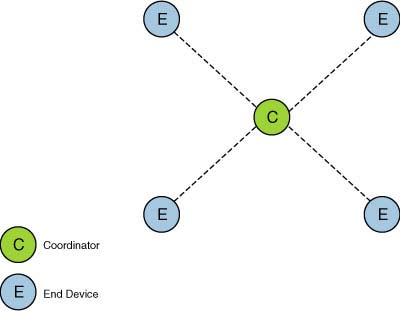
\includegraphics[width=0.45\textwidth]{Images/Star.png}
    \caption{Star topology -- Thiết bị kết nối qua Coordinator trung tâm}
    \label{fig:ch2-zigbee-star}
\end{figure}
\noindent Ưu điểm của hình sao là dễ quản lý, trễ truyền dẫn nhỏ nhưng nhược điểm lớn là vùng phủ sóng bị giới hạn bởi công suất phát của một node Coordinator và Coordinator trở thành điểm lỗi duy nhất của toàn hệ thống (single point of failure).

Mạng lưới (Mesh Topology) được thể hiện trong Hình \ref{fig:ch2-zigbee-mesh}, là cấu trúc mạnh mẽ nhất của chuẩn Zigbee. Các node Router có khả năng tự động liên kết nối mạng với nhau tạo thành mạng lưới truyền dẫn điểm-điểm đa chặng (multi-hop routing).
\begin{figure}[H]
    \centering
    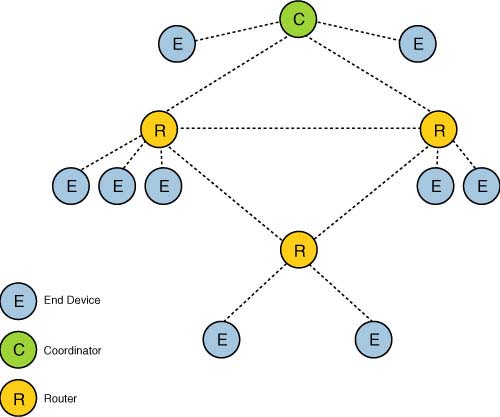
\includegraphics[width=0.45\textwidth]{Images/Mesh.png}
    \caption{Mesh topology -- Định tuyến đa chặng linh hoạt}
    \label{fig:ch2-zigbee-mesh}
\end{figure}
\noindent Khi một chặng liên kết giữa hai node Router bị lỗi vật lý (do cản trở hoặc nhiễu sóng), thuật toán định tuyến AODV tích hợp sẵn trong NWK layer sẽ tự động tìm kiếm đường đi thay thế khác để truyền đạt thông tin tới đích, đảm bảo hệ thống tự phục hồi (self-healing).

Mạng hình cây (Tree Topology) được mô phỏng trong Hình \ref{fig:ch2-zigbee-tree}, là cấu trúc phân cấp hình cây trong đó Coordinator là gốc, các Router đóng vai trò nhánh cây trung gian và End Device là lá cây ở cấp thấp nhất.
\begin{figure}[H]
    \centering
    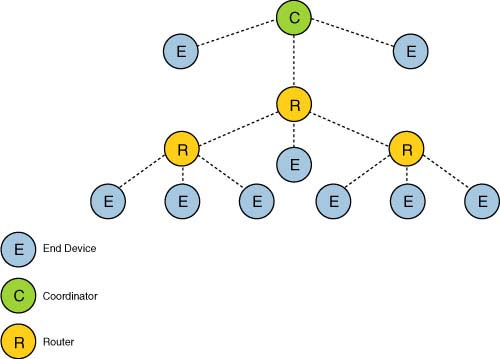
\includegraphics[width=0.45\textwidth]{Images/Tree.png}
    \caption{Tree topology -- Cấu trúc phân cấp hình cây}
    \label{fig:ch2-zigbee-tree}
\end{figure}
\noindent Topo này kết hợp sự đơn giản trong định địa chỉ của topo hình sao và khả năng mở rộng khoảng cách của topo mạng lưới, phù hợp cho các mô hình quản lý phân lớp trong tòa nhà. Trong đồ án này, hệ thống triển khai thực tế theo cấu hình mạng mesh-tree linh hoạt.

\subsection{Kiến trúc Protocol Stack}
\label{sec:ch2-zigbee-layers}

Kiến trúc phân tầng của giao thức Zigbee được xây dựng trên nền tảng chuẩn vật lý IEEE 802.15.4 như được mô tả chi tiết trong Hình \ref{fig:ch2-zigbee-stack}.

\begin{figure}[H]
    \centering
    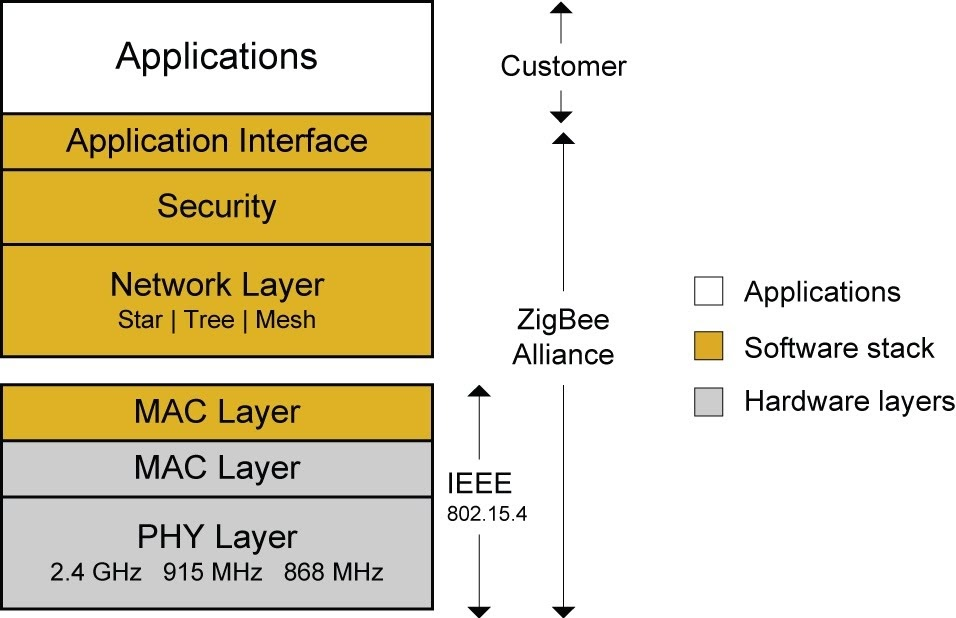
\includegraphics[width=0.5\textwidth]{Images/Zigbee_Architecture.png}
    \caption{Kiến trúc phân tầng Zigbee Protocol Stack}
    \label{fig:ch2-zigbee-stack}
\end{figure}

Sự phân chia chức năng giữa các lớp trong stack bao gồm:
\textbf{Lớp PHY (Physical Layer):} Được định nghĩa bởi chuẩn IEEE 802.15.4, chịu trách nhiệm truyền phát các bit dữ liệu trên dải sóng vô tuyến tần số 2.4 GHz, thực hiện điều chế tín hiệu DSSS (Direct Sequence Spread Spectrum) và đo năng lượng kênh (LQI).

\textbf{Lớp MAC (Medium Access Control):} Quản lý việc truy cập kênh vô tuyến chung sử dụng cơ thức CSMA-CA (Carrier Sense Multiple Access with Collision Avoidance), kiểm soát lỗi truyền tin cậy qua cơ chế ACK và định dạng cấu trúc khung truyền MAC.

\textbf{Lớp NWK (Network Layer):} Do Zigbee Alliance định nghĩa, phụ trách cấp phát địa chỉ mạng 16-bit động cho thiết bị khi gia nhập mạng, xây dựng bảng định tuyến và bảo mật tầng mạng bằng Network Key dùng chung.

\textbf{Lớp APS (Application Support Sublayer):} Cầu nối trung gian giữa lớp mạng NWK và lớp ứng dụng ZCL. APS phụ trách lọc các bản tin trùng lặp, duy trì Bảng Binding (liên kết trực tiếp) và thực hiện phân mảnh bản tin nếu kích thước dữ liệu vượt quá giới hạn MTU (127 bytes).

\textbf{Lớp ZCL (Zigbee Cluster Library):} Định nghĩa mô hình trao đổi dữ liệu hướng đối tượng (cluster/attribute/command) giúp chuẩn hóa hành vi ứng dụng của thiết bị.

\subsection{Địa chỉ và bảo mật trong mạng}
\label{sec:ch2-zigbee-address}

Mỗi thiết bị Zigbee sở hữu hai loại địa chỉ phân biệt để phục vụ truyền thông:
\textbf{Địa chỉ vật lý EUI-64 (Extended Unique Identifier):} Là địa chỉ MAC 64-bit cố định duy nhất được nhà sản xuất nạp sẵn vào chip bán dẫn. Địa chỉ này được đồ án sử dụng làm khóa định danh duy nhất (primary key) để xác định thiết bị trên MQTT và cơ sở dữ liệu Cloud, đảm bảo tính nhất quán ngay cả khi thiết bị ngắt kết nối vật lý.

\textbf{Địa chỉ mạng 16-bit (NwkAddr):} Là địa chỉ runtime được Coordinator cấp phát động cho thiết bị khi gia nhập mạng. Địa chỉ này có thể thay đổi sau mỗi lần thiết bị khởi động lại hoặc thực hiện rejoin mạng, do đó chỉ được dùng cho mục đích định tuyến lớp thấp của stack Zigbee và không được dùng làm primary key trên database.

Bảo mật mạng được kiểm soát thông qua hai loại khóa chính: Network Key 128-bit dùng để mã hóa toàn bộ dữ liệu truyền trên không trung ở tầng NWK và Link Key 128-bit dùng để mã hóa kênh truyền bảo mật điểm-điểm giữa Coordinator/Trust Center và một thiết bị cụ thể khi trao đổi Network Key.

\subsection{Quá trình hình thành và gia nhập mạng}
\label{sec:ch2-zigbee-join-process}

Mạng được hình thành khi Gateway ra lệnh cho Coordinator (chạy firmware NCP) khởi chạy quét năng lượng vô tuyến để tự động chọn kênh tần số ít nhiễu nhất trong số 16 kênh từ kênh 11 đến 26. Sau khi thiết lập mạng thành công với một ID mạng PAN ID ngẫu nhiên không trùng lặp, Gateway ra lệnh mở cửa sổ permit-join trong một khoảng thời gian giới hạn (ví dụ 60 giây).

Quá trình thiết bị con (End Device hoặc Router) gia nhập mạng diễn ra qua bốn bước cụ thể sau:
\textbf{Bước 1 -- Khám phá mạng (Network Discovery):} Thiết bị con phát quảng bá tin nhắn Beacon Request để quét các mạng xung quanh. Coordinator nhận được tin nhắn và phản hồi lại bằng Beacon Frame chứa thông tin PAN ID và trạng thái cho phép gia nhập mạng (Association Permit = True).

\textbf{Bước 2 -- Kết nối vật lý (MAC Association):} Thiết bị con gửi yêu cầu kết nối MAC Association Request chứa địa chỉ EUI-64 và khả năng phần cứng (node capability). Coordinator phê duyệt và cấp phát một địa chỉ mạng 16-bit ngẫu nhiên thông qua bản tin MAC Association Response.

\textbf{Bước 3 -- Xác thực bảo mật và trao đổi khóa:} Coordinator (Trust Center) mã hóa Network Key hiện tại bằng Link Key mặc định (chẳng hạn Link Key tiêu chuẩn \texttt{ZigbeeAlliance09}) và gửi xuống thiết bị con qua bản tin Transport Key. Thiết bị con nhận, giải mã để lấy Network Key và lưu trữ.

\textbf{Bước 4 -- Cập nhật và Thông báo (Device Announce):} Thiết bị con phát quảng bá bản tin Device Announce chứa địa chỉ EUI-64 và địa chỉ mạng 16-bit mới của nó để thông báo cho toàn mạng biết sự hiện diện của mình. Lúc này, Gateway sẽ bắt sự kiện này để cập nhật bảng lưu trữ cục bộ.

% ========================================
% 2.3 ZIGBEE CLUSTER LIBRARY (ZCL)
% ========================================
\section{Thư viện cluster Zigbee Cluster Library (ZCL)}
\label{sec:ch2-zcl}

ZCL đóng vai trò là một chuẩn mô tả dữ liệu ở lớp ứng dụng, định nghĩa hành vi và định dạng trao đổi thông tin thống nhất giữa các thiết bị thuộc nhiều nhà sản xuất khác nhau.

\subsection{Cấu trúc mô hình ZCL}
\label{sec:ch2-zcl-structure}

Mô hình ZCL tổ chức dữ liệu theo kiến trúc hướng đối tượng, bao gồm:
\textbf{Cluster (Cụm chức năng):} Là đơn vị logic gom nhóm các thuộc tính và lệnh điều khiển có liên quan chặt chẽ tới một chức năng vật lý cụ thể (ví dụ: On/Off Cluster, Temperature Measurement Cluster). Mỗi cluster được gán một mã ID 16-bit duy nhất.

\textbf{Attribute (Thuộc tính):} Các biến lưu trữ trạng thái thực tế của thiết bị bên trong một cluster (ví dụ: thuộc tính \texttt{OnOff} kiểu Boolean lưu trạng thái bật/tắt của đèn, thuộc tính \texttt{MeasuredValue} lưu giá trị nhiệt độ đo được).

\textbf{Command (Lệnh điều khiển):} Các hành động tác động gửi tới thiết bị để thay đổi thuộc tính hoặc yêu cầu thiết bị thực thi một tác vụ (ví dụ: lệnh \texttt{Toggle} gửi tới On/Off cluster để đảo trạng thái thuộc tính \texttt{OnOff}).

ZCL phân chia rõ ràng vai trò Client và Server. Server cluster là nơi lưu giữ giá trị thực tế của các thuộc tính (ví dụ: bóng đèn chứa On/Off Server Cluster chứa biến trạng thái của rơ-le đèn). Client cluster là nơi gửi đi các lệnh điều khiển thuộc tính hoặc truy vấn thuộc tính (ví dụ: công tắc chứa On/Off Client Cluster để gửi lệnh bật/tắt đi). Sự phối hợp Client/Server được mô phỏng trong Hình \ref{fig:ch2-zcl-client-server}.

\begin{figure}[H]
    \centering
    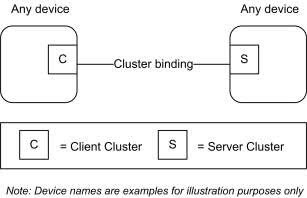
\includegraphics[width=0.55\textwidth]{Images/Client_Server_Model.png}
    \caption{Mô hình tương tác Client/Server trong ZCL}
    \label{fig:ch2-zcl-client-server}
\end{figure}

\subsection{Cơ chế Binding (Liên kết)}
\label{sec:ch2-zcl-binding}

Binding là cơ chế cốt lõi của lớp APS cho phép thiết lập liên kết trực tiếp giữa hai endpoint của hai thiết bị Zigbee (ví dụ: liên kết từ On/Off Client của Switch tới On/Off Server của Light). Khi Bảng Binding được thiết lập thành công trên Coordinator, Switch có thể phát lệnh gửi đi trực tiếp thông qua địa chỉ logic của liên kết mà không cần ghi rõ địa chỉ 16-bit của Light. Cơ chế này giúp thiết bị công tắc bật/tắt đèn trực tiếp trong mạng cục bộ mà không cần sự can thiệp hay xử lý của phần mềm Gateway hoặc Cloud, giảm độ trễ tối đa và đảm bảo hệ thống vận hành tự động cục bộ khi mất kết nối mạng WAN.

% ========================================
% 2.4 GATEWAY TRONG HỆ THỐNG IoT
% ========================================
\section{Vai trò của Gateway trong hệ thống IoT}
\label{sec:ch2-gateway}

Gateway đóng vai trò là phần tử biên (Edge Device) chuyển đổi giao thức truyền thông hai chiều giữa lớp vô tuyến cục bộ RF và lớp mạng IP diện rộng.

Gateway thu nhận các bản tin báo cáo thuộc tính ZCL (ZCL Attribute Reports) nhận từ thiết bị Zigbee qua UART/EZSP, phân tích dữ liệu nhị phân thô, sau đó chuyển đổi và đóng gói thành bản tin JSON tiêu chuẩn. JSON payload này được publish lên các MQTT topics tương ứng để Cloud xử lý. Ở chiều ngược lại, Gateway lắng nghe các yêu cầu điều khiển từ Cloud qua MQTT, giải mã và dispatch lệnh thành gói tin EZSP để Coordinator truyền xuống thiết bị đích.

% ========================================
% 2.5 GIAO THỨC TRUYỀN THÔNG MQTT
% ========================================
\section{Giao thức truyền thông MQTT}
\label{sec:ch2-mqtt}

MQTT (Message Queuing Telemetry Transport) là giao thức truyền thông điệp gọn nhẹ hoạt động theo mô hình Publish/Subscribe chạy trên nền tảng TCP/IP.

\subsection{Kiến trúc Publish/Subscribe}
\label{sec:ch2-mqtt-pubsub}

Mô hình publish/subscribe của MQTT loại bỏ hoàn toàn sự kết nối trực tiếp giữa các máy khách gửi dữ liệu (Publishers) và máy khách nhận dữ liệu (Subscribers) bằng cách sử dụng một máy chủ trung gian gọi là Broker (Mosquitto Broker). Khi một client publish tin nhắn tới một chủ đề cụ thể (Topic), Broker sẽ nhận bản tin đó và chịu trách nhiệm phân phối bản tin đến tất cả các clients đã đăng ký lắng nghe chủ đề đó như được thể hiện trong Hình \ref{fig:ch2-mqtt-flow}.

\begin{figure}[H]
    \centering
    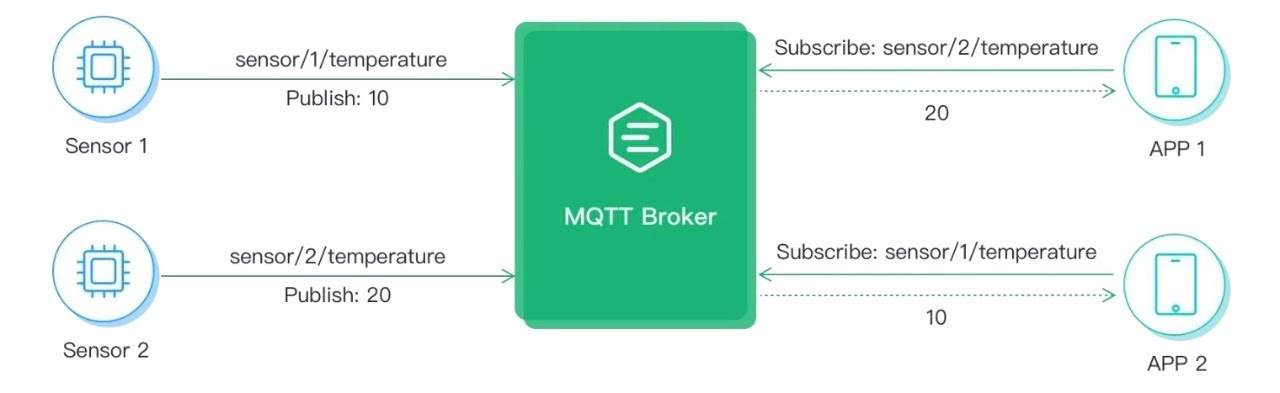
\includegraphics[width=0.75\textwidth]{Images/MQTT_pub-sub.png}
    \caption{Kiến trúc truyền thông Publish/Subscribe qua Broker trung gian}
    \label{fig:ch2-mqtt-flow}
\end{figure}

\subsection{Quality of Service (QoS) trong MQTT}
\label{sec:ch2-mqtt-qos}

MQTT định nghĩa ba mức đảm bảo chất lượng dịch vụ (QoS) nhằm cân bằng giữa độ tin cậy truyền dẫn và băng thông đường truyền:
\textbf{QoS 0 (At most once):} Broker hoặc client gửi tin nhắn một lần duy nhất và không yêu cầu xác nhận. Tin nhắn có thể bị mất nếu mạng không ổn định, nhưng đây là mức nhanh nhất và tốn ít băng thông nhất. Phù hợp cho các bản tin telemetry báo cáo nhiệt độ định kỳ.

\textbf{QoS 1 (At least once):} Đảm bảo tin nhắn được truyền đến đích ít nhất một lần qua cơ chế xác nhận gói tin (PUBACK). Nếu bên gửi không nhận được PUBACK sau khoảng thời gian timeout, nó sẽ gửi lại tin nhắn (dẫn tới nguy cơ trùng lặp bản tin). Đồ án sử dụng mức QoS 1 cho toàn bộ luồng command và state reported quan trọng.

\textbf{QoS 2 (Exactly once):} Đảm bảo tin nhắn đến đích đúng một lần duy nhất thông qua quá trình bắt tay bốn bước phức tạp. Đây là mức chậm nhất và tốn băng thông nhất, không được sử dụng trong hệ thống demo của đồ án.

\subsection{Retained Messages và Last Will and Testament (LWT)}
\label{sec:ch2-mqtt-features}

\textbf{Retained Message (Tin nhắn lưu trữ):} Khi publish một bản tin với cờ Retain được set bằng True, Broker sẽ lưu trữ bản tin cuối cùng của topic đó. Khi một subscriber mới đăng ký topic đó, Broker sẽ lập tức gửi ngay bản tin lưu trữ này xuống, giúp subscriber mới cập nhật ngay trạng thái hiện tại của thiết bị mà không cần chờ thiết bị phát báo cáo chu kỳ tiếp theo.

\textbf{Last Will and Testament (LWT - Di chúc):} LWT cho phép một client khi kết nối với Broker đăng ký một bản tin mặc định cùng topic tương ứng. Nếu client bị ngắt kết nối đột ngột không mong muốn (ví dụ mất nguồn điện Gateway), Broker sẽ tự động publish bản tin "di chúc" này để thông báo cho hệ thống Cloud biết thiết bị Gateway đã đi vào trạng thái offline.

% ========================================
% 2.6 GIAO TIẾP NỐI TIẾP UART
% ========================================
\section{Giao tiếp nối tiếp UART}
\label{sec:ch2-uart}

UART (Universal Asynchronous Receiver/Transmitter) là giao thức truyền thông nối tiếp bất đồng bộ, sử dụng hai đường dây tín hiệu TX (truyền) và RX (nhận) để thực hiện kết nối vật lý point-to-point trực tiếp giữa host Linux chạy Z3Gateway và chip NCP EFR32MG12 như trong Hình \ref{fig:ch2-uart}.

\begin{figure}[H]
    \centering
    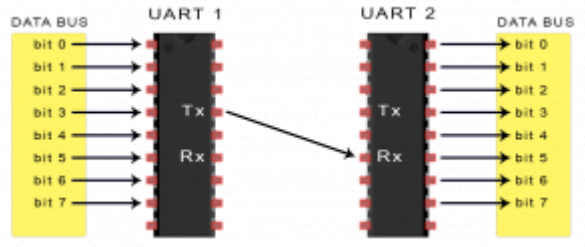
\includegraphics[width=0.55\textwidth]{Images/UART.png}
    \caption{Kết nối UART vật lý giữa Host và NCP}
    \label{fig:ch2-uart}
\end{figure}

Giao tiếp UART bất đồng bộ yêu cầu hai bên thống nhất cấu hình tốc độ truyền (Baud rate), bit dữ liệu, bit dừng (Stop bit) và bit kiểm tra chẵn lẻ (Parity). Trong đồ án, UART kết nối Host-NCP hoạt động ở baud rate mặc định 115200 bps, kết hợp giao thức ASH (Asynchronous Serial Host) do Silicon Labs đặc tả để đóng khung dữ liệu (framing), kiểm tra lỗi CRC và điều khiển luồng (flow control) nhằm bảo vệ tính toàn vẹn của các khung lệnh EZSP.

% ========================================
% 2.7 PHẦN CỨNG VÀ KIT SỬ DỤNG
% ========================================
\section{Phần cứng và Kit phát triển sử dụng}
\label{sec:ch2-hardware}

Để triển khai các node thiết bị thực tế, đồ án sử dụng bộ công cụ phát triển phần cứng chuyên nghiệp của hãng Silicon Labs.

\subsection{Wireless Starter Kit BRD4001A và BRD4162A}
\label{sec:ch2-starter-kit}

Thiết bị phần cứng cốt lõi được sử dụng là kit phát triển EFR32MG12 2.4 GHz 10 dBm Wireless Starter Kit (WSTK) như được chụp lại trong Hình \ref{fig:ch2-kit-photo}.

\begin{figure}[H]
    \centering
    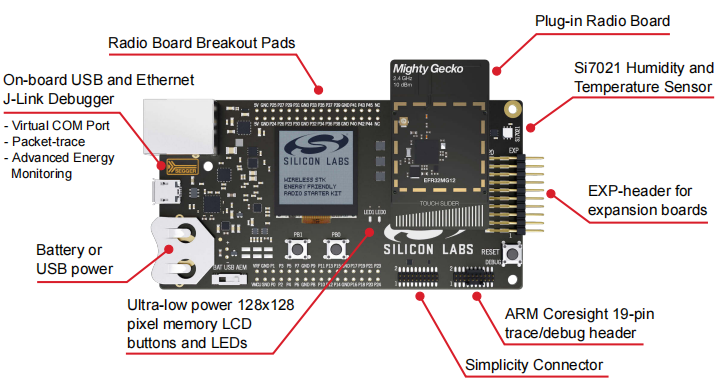
\includegraphics[width=0.75\textwidth]{Images/Kit.png}
    \caption{Hình ảnh bộ kit phát triển EFR32MG12 Wireless Starter Kit}
    \label{fig:ch2-kit-photo}
\end{figure}

Bộ kit phát triển bao gồm hai thành phần bo mạch lắp ghép chính:
\textbf{Radio Board BRD4162A:} Là bo mạch cắm chứa SoC EFR32MG12P332F1024GL125 chuyên dụng cho truyền thông không dây đa giao thức (Wireless Gecko). Chip bán dẫn này tích hợp lõi vi xử lý ARM Cortex-M4 32-bit tốc độ 40 MHz, dung lượng bộ nhớ Flash 1024 kB phục vụ lưu trữ firmware, bộ nhớ RAM 256 kB và mạch thu phát vô tuyến công suất phát tối đa +10 dBm trên băng tần 2.4 GHz kèm anten mạch in PCB anten tích hợp.

\textbf{Mainboard BRD4001A:} Là bo mạch mẹ cung cấp mạch nạp Segger J-Link tích hợp để gỡ lỗi mã nguồn, màn hình LCD hiển thị thông tin, cảm biến đo nhiệt độ Si7021, cùng các nút nhấn vật lý (BTN0, BTN1) và đèn LED (LED0, LED1) để lập trình mô phỏng thiết bị.

\subsection{Cấu hình phần cứng theo vai trò ứng dụng}
\label{sec:ch2-hw-mapping}

Các board phần cứng EFR32MG12 được lập trình nạp firmware riêng biệt để mô phỏng bốn thành phần vật lý của mạng Zigbee:
\textbf{Coordinator/NCP Board:} Cắm trực tiếp vào host qua cổng USB để thiết lập kết nối VCOM UART ảo, chạy firmware NCP thuần để làm bộ thu phát sóng Zigbee cho gateway.

\textbf{Z3Light Board:} Sử dụng LED0 trên Mainboard để mô phỏng trạng thái bóng đèn (LED0 sáng tương ứng đèn ON, LED0 tắt tương ứng đèn OFF).

\textbf{Z3Switch Board:} Sử dụng nút nhấn BTN0 trên Mainboard để gửi lệnh Toggle thay đổi trạng thái của đèn qua binding.

\textbf{Occupancy Sensor Board:} Cấu hình ở chế độ Sleepy End Device chạy nguồn pin, sử dụng nút nhấn BTN0 để mô phỏng sự kiện cảm biến phát hiện có người di chuyển.
